\documentclass[journal,oneside,a4paper,onecolumn]{IEEEtran}

% Some very useful LaTeX packages include:
% (uncomment the ones you want to load)

% *** CITATION PACKAGES ***
%
\usepackage{cite}
% cite.sty was written by Donald Arseneau
% V1.6 and later of IEEEtran pre-defines the format of the cite.sty package
% \cite{} output to follow that of IEEE. Loading the cite package will
% result in citation numbers being automatically sorted and properly
% "compressed/ranged". e.g., [1], [9], [2], [7], [5], [6] without using
% cite.sty will become [1], [2], [5]--[7], [9] using cite.sty. cite.sty's
% \cite will automatically add leading space, if needed. Use cite.sty's
% noadjust option (cite.sty V3.8 and later) if you want to turn this off.
% cite.sty is already installed on most LaTeX systems. Be sure and use
% version 4.0 (2003-05-27) and later if using hyperref.sty. cite.sty does
% not currently provide for hyperlinked citations.
% The latest version can be obtained at:
% http://www.ctan.org/tex-archive/macros/latex/contrib/cite/
% The documentation is contained in the cite.sty file itself.


% *** GRAPHICS RELATED PACKAGES ***
%
  \usepackage{graphicx}
  \graphicspath{{figs/}}
  \DeclareGraphicsExtensions{.pdf,.png}
  \usepackage{color}

% *** MATH PACKAGES ***
%
\usepackage[cmex10]{amsmath}
% A popular package from the American Mathematical Society that provides
% many useful and powerful commands for dealing with mathematics. If using
% it, be sure to load this package with the cmex10 option to ensure that
% only type 1 fonts will utilized at all point sizes. Without this option,
% it is possible that some math symbols, particularly those within
% footnotes, will be rendered in bitmap form which will result in a
% document that can not be IEEE Xplore compliant!
%
% Also, note that the amsmath package sets \interdisplaylinepenalty to 10000
% thus preventing page breaks from occurring within multiline equations. Use:
%\interdisplaylinepenalty=2500
% after loading amsmath to restore such page breaks as IEEEtran.cls normally
% does. amsmath.sty is already installed on most LaTeX systems. The latest
% version and documentation can be obtained at:
% http://www.ctan.org/tex-archive/macros/latex/required/amslatex/math/

%\usepackage{amssymb}%............................ AMS Symbol fonts



% *** SPECIALIZED LIST PACKAGES ***
%
%\usepackage{algorithmic}
% algorithmic.sty was written by Peter Williams and Rogerio Brito.
% This package provides an algorithmic environment for describing algorithms.
% You can use the algorithmic environment in-text or within a figure
% environment to provide for a floating algorithm. Do NOT use the algorithm
% floating environment provided by algorithm.sty (by the same authors) or
% algorithm2e.sty (by Christophe Fiorio) as IEEE does not use dedicated
% algorithm float types and packages that provide these will not provide
% correct IEEE style captions. The latest version and documentation of
% algorithmic.sty can be obtained at:
% http://www.ctan.org/tex-archive/macros/latex/contrib/algorithms/
% There is also a support site at:
% http://algorithms.berlios.de/index.html
% Also of interest may be the (relatively newer and more customizable)
% algorithmicx.sty package by Szasz Janos:
% http://www.ctan.org/tex-archive/macros/latex/contrib/algorithmicx/

% *** ALIGNMENT PACKAGES ***
%
\usepackage{array}
% Frank Mittelbach's and David Carlisle's array.sty patches and improves
% the standard LaTeX2e array and tabular environments to provide better
% appearance and additional user controls. As the default LaTeX2e table
% generation code is lacking to the point of almost being broken with
% respect to the quality of the end results, all users are strongly
% advised to use an enhanced (at the very least that provided by array.sty)
% set of table tools. array.sty is already installed on most systems. The
% latest version and documentation can be obtained at:
% http://www.ctan.org/tex-archive/macros/latex/required/tools/


\usepackage{mdwmath}
\usepackage{mdwtab}
% Also highly recommended is Mark Wooding's extremely powerful MDW tools,
% especially mdwmath.sty and mdwtab.sty which are used to format equations
% and tables, respectively. The MDWtools set is already installed on most
% LaTeX systems. The lastest version and documentation is available at:
% http://www.ctan.org/tex-archive/macros/latex/contrib/mdwtools/

% IEEEtran contains the IEEEeqnarray family of commands that can be used to
% generate multiline equations as well as matrices, tables, etc., of high
% quality.

% *** SUBFIGURE PACKAGES ***
% subfig.sty, also written by Steven Douglas Cochran, is the modern
% replacement for subfigure.sty. However, subfig.sty requires and
% automatically loads Axel Sommerfeldt's caption.sty which will override
% IEEEtran.cls handling of captions and this will result in nonIEEE style
% figure/table captions. To prevent this problem, be sure and preload
% caption.sty with its "caption=false" package option. This is will preserve
% IEEEtran.cls handing of captions. Version 1.3 (2005/06/28) and later
% (recommended due to many improvements over 1.2) of subfig.sty supports
% the caption=false option directly:
\usepackage[caption=false,font=footnotesize]{subfig}
%
% The latest version and documentation can be obtained at:
% http://www.ctan.org/tex-archive/macros/latex/contrib/subfig/
% The latest version and documentation of caption.sty can be obtained at:
% http://www.ctan.org/tex-archive/macros/latex/contrib/caption/

%Setting captions to centered (Not IEEE journal standard)
\makeatletter
\long\def\@makecaption#1#2{\ifx\@captype\@IEEEtablestring%
\footnotesize\begin{center}{\normalfont\footnotesize #1}\\
{\normalfont\footnotesize\scshape #2}\end{center}%
\@IEEEtablecaptionsepspace
\else
\@IEEEfigurecaptionsepspace
\setbox\@tempboxa\hbox{\normalfont\footnotesize {#1.}~~ #2}%
\ifdim \wd\@tempboxa >\hsize%
\setbox\@tempboxa\hbox{\normalfont\footnotesize {#1.}~~ }%
\parbox[t]{\hsize}{\normalfont\footnotesize \noindent\unhbox\@tempboxa#2}%
\else
\hbox to\hsize{\normalfont\footnotesize\hfil\box\@tempboxa\hfil}\fi\fi}
\makeatother


% *** FLOAT PACKAGES ***
%
\usepackage{fixltx2e}
% fixltx2e, the successor to the earlier fix2col.sty, was written by
% Frank Mittelbach and David Carlisle. This package corrects a few problems
% in the LaTeX2e kernel, the most notable of which is that in current
% LaTeX2e releases, the ordering of single and double column floats is not
% guaranteed to be preserved. Thus, an unpatched LaTeX2e can allow a
% single column figure to be placed prior to an earlier double column
% figure. The latest version and documentation can be found at:
% http://www.ctan.org/tex-archive/macros/latex/base/

% *** PDF, URL AND HYPERLINK PACKAGES ***
%
\usepackage{url}

\usepackage{sistyle}
    \SIstyle{S-Africa}
    \SIunitspace{{\cdot}}
    \SIunitdot{{\cdot}}

% generate nice bookmarks and hyperrefs when exporting to pdf and dvi (screen version):
\usepackage[a4paper,plainpages=false,colorlinks,linktocpage,bookmarks=true,bookmarksopen=false]{hyperref}
% use this for printing only (no color, print version):
%\usepackage[a4paper,plainpages=false,colorlinks=false,linktocpage,bookmarks=true,bookmarksopen=false]{hyperref}

% correct bad hyphenation here
\hyphenation{op-tical net-works semi-conduc-tor}

%List of acronyms used in text
 \usepackage{acronym}%.......................... Acronym package to handle acronyms in text

\acrodef{MMOG}{Massively Multiplayer Online Game}
\acrodef{MMORPG}{Massively Multiplayer Online Role Playing Game}
\acrodef{WoW}{World of Warcraft}
\acrodef{MUD}{Multi-User Dungeon}
\acrodef{PvP}{Player-versus-Player}

\begin{document}

%
% paper title
\title{A Scalable Distributed Peer-to-Peer MMOG Architecture}

\author{\IEEEauthorblockN{John S. Gilmore\\}
\IEEEauthorblockA{Department of Electronic Engineering\\
Stellenbosch University\\
Stellenbosch, South Africa\\
Email: jgilmore@ieee.org}}

% make the title area
\maketitle

\begin{abstract}
%\boldmath
The abstract goes here.
\end{abstract}

\hfill May, 2010

\section{Introduction}


\IEEEPARstart{W}{ith} the advent of broadband Internet, \acp{MMOG} have gained significant popularity over the course of the past few years.
Figure \ref{fig_mmog_subscriptions} shows the total number of active MMOG subscriptions over time for the period 1997 to 2008. From here, the accelerating growth of the MMOG market is evident.
%
\begin{figure}[htbp]
 \centering
 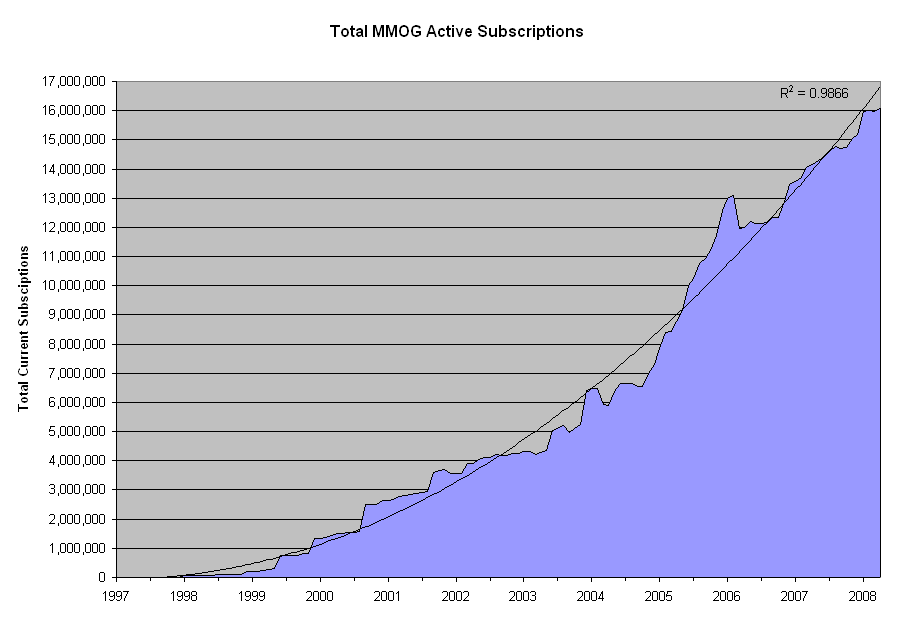
\includegraphics[width=0.5\columnwidth]{MMOG_subscriptions}
 \caption{Total number of active MMOG player subscriptions over time \cite{mmo_growth_chart}.}
 \label{fig_mmog_subscriptions}
\end{figure}

\acp{MMOG} are characterised by expansive worlds, where a large number of players interact online with each other and the virtual environment to achieve certain goals through collaboration and teamwork. Throughout the development of \acp{MMOG}, role play has been tightly coupled to this type of game. This is perhaps due to the exploration and player interaction aspects. Role play allows players to fully immerse themselves in the game world and might, therefore, provide for a more compelling experience. Because of this tight coupling, the terms \ac{MMORPG} and \ac{MMOG} have almost become synonymous. Throughout this work, a distinction will, however, be made between the two.

\acp{MMOG} hold great commercial as well as academic value. From a commercial perspective, the growing number of active subscriptions shown in Figure \ref{fig_mmog_subscriptions} translates to a growing \ac{MMOG} market. Figure \ref{fig_mmog_market} shows the online games market forecast by DFC Intelligence, a company specialising in game market forecasts for various sectors.
%
\begin{figure}[htbp]
 \centering
 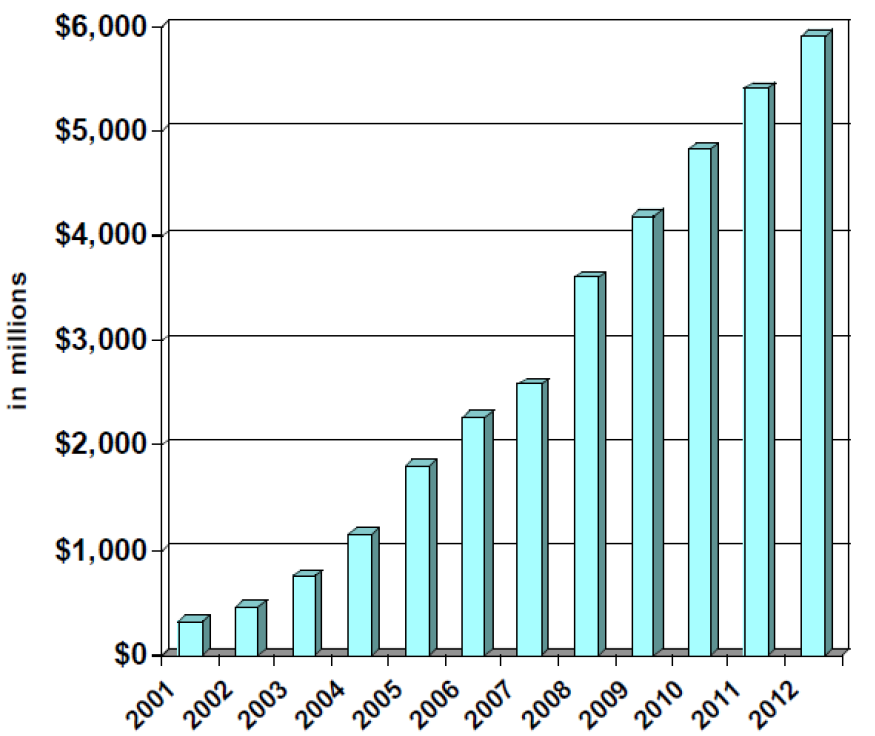
\includegraphics[width=0.5\columnwidth]{DFC_MMOG_market}
 \caption{DFC Intelligence MMOG market forecast '08 \cite{Fan_phd}.}
 \label{fig_mmog_market}
\end{figure}

From an academic perspective, \acp{MMOG} also hold great value. An MMOG is a complex networked application, with clients requiring reliable real-time feedback on actions taken. The design of an MMOG requires in-depth knowledge of server architectures and network design. The design of a server architecture determines how may players the game will be able to host and what the user experience will be in terms of quality of service. The server architecture must be able to handle thousands of requests, store large amounts of data, update the game state and send responses back to all clients in real time.

\subsection{A brief history of MMORPGs}

\acp{MMOG} have a history stretching from 1978 to the present. A complete history of \acp{MMOG} and the histories of the games and boardgames that they originate from can be found in \cite{mmog_past_present_future} and Chapter 1 of \cite{designing_virtual_worlds}. The first games that could be called \acp{MMOG} were \acp{MUD} (1978) \cite{mud_intro}. \acp{MUD} are entirely text-based, with players exploring areas by receiving descriptions of what they were ``seeing'' and typing commands to move and interact with objects or players. \acp{MUD} contain many of the elements that today are still central to the \ac{MMOG} concept. These elements include exploration, large worlds, multiplayer, social interaction and progression.

After \acp{MUD}, there were many \acp{MMORPG} that acted as building blocks for what is recognised today as being an \ac{MMORPG}. The first graphical \ac{MMORPG} was Neverwinter Nights (1991) \cite{nwn_aol}. Neverwinter Nights was not an Internet based game, it was hosted on what today is the AOL network. Meridian 59 (1994) was the first \ac{MMOG} to have featured a monthly subscription fee, receive wide media coverage and most importantly, the first \ac{MMOG} to feature a 3D engine \cite{meridian59_hist}.

The first \ac{MMORPG} to be commercially successful and largely credited with popularising the genre was Ultima Online (1997). Ultima Online used existing intellectual property from the Ultima universe as well as an aggressive marketing campaign by game publisher EA, to quickly gain 100,000 subscribers. NCsoft's Lineage (1998) looked similar to Ultima Online, but was more \ac{PvP} oriented and with an added castle siege mechanism, became very popular in South Korea. Lineage had more than three million subscribers at one point, most of them from South Korea \cite{mmog_subscriptions}. Everquest (1999) is credited for bringing \acp{MMORPG} into mainstream Western Culture. It featured a large persistent 3D environment that was capable of hosting up to 15000 players per server \cite{everquest2_capacity}.

\acp{MMORPG} in the first millennium are considered to be of the first generation. These games provided blueprints for all \acp{MMORPG}
to follow in the second generation. While there are many more games in the second generation, these games are characterised by little innovation
in the genre and focus more on improving graphics and ease-of-use \cite{mmog_past_present_future}. Notable games in this generation are: Final Fantasy XI (2000) (console based), Dark Age of Camelot (2001) (realm vs. realm combat) and Anarchy Online (2001) (instancing).

Eve Online (2003), developed by CCP Games in Iceland, brought many new innovations to the \ac{MMORPG}. It was the first successful MMORPG to feature a science fiction theme. It was the first MMOG to have a single distributed server architecture. This meant that no sharding was required. Sharding is a method by which the game world is duplicated onto multiple servers to distribute load. Players cannot communicate between shards as these worlds are complectly isolated from each other. By employing a distributed server architecture, where different regions of the virtual world was hosted on different servers, players could have a seamless and more immersive experience. This was accomplished by hosting different star systems on different servers. Players have to use a warp gate to travel between star systems. This mechanic is used to mask the time it takes to move the player from one server to another. In 2006, CCP Games launched the largest supercomputer in the gaming industry to upgrade their existing infrastructure and enable Eve to support more than 50,000 concurrent users \cite{eve_launces_supcom}. This number that was surpassed in 2009 with 54,181 concurrent users in game \cite{eve_pcu}.

Another innovation of Eve was the in-game economy. CCP games appointed Dr. Eyj\'{o}lfur Gu\~{o}mundsson as chief economist of Eve online in 2006 \cite{eve_economist}. His duties were to monitor and predict market trends in the game world and produce detailed quarterly economic reports \cite{eve_econ_rep}.  The economy is based on a open market system ruled by supply and demand. No other game has implemented an in-game economy in such a rigourous fashion.

Blizzards's \ac{WoW} (2004) is the most successful MMORPG to date. After six years it still has by far the most subscribers of any MMOG, totaling 11,5 million, each paying \$15 per month subscription \cite{wow_subscibers}. In 2008 it was estimated that WoW holds more than 60\% of the MMORPG subscription market \cite{mmog_sub_market}. From the first generation of games, a steady growth has been seen in the MMOG space, but before the run away success of WoW, no one had estimated that the gaming market could be this large \cite{mmog_growth_analysis}. It should be noted, however, that the growth seen in the \ac{MMOG} market, is mostly due to growth in the Asian markets and that the size of these markets are much larger than the size of the Western markets.

The success of \ac{WoW} has largely been attributed to the overall quality and finish of the game \cite{wow_csf}. It is interesting to note that WoW is not attributed with many innovations. Most games that came before it implemented most of the features in WoW. What WoW did do, is combine all previous innovations into a package that was accessible to a large number of people.  Players also don't just play WoW to experience the game content, they also play the game to meet up with friends and socialise. Guilds are also an integral part of WoW. Guilds are collections of players that choose to play together to achieve some common goal.

\section{Overview of MMOG network architectures}

The previous section presented a brief history of the \ac{MMOG} and more specifically, the \ac{MMORPG} genre. This section explores the network architecture that is generally employed by this genre of games. The network architecture of a system specifies how the different entities in the network communicate. On a high level, there are two well-known general network architectures: The client/server model and the peer-to-peer model. Bear in mind that these models are not specific to MMOGS, what is specific to them is how the models are implemented to store and disseminate data. These models specify how data are distributed over the network and what the levels of control are that each entity in the network possesses.

\begin{figure}[htbp]
 \centering
 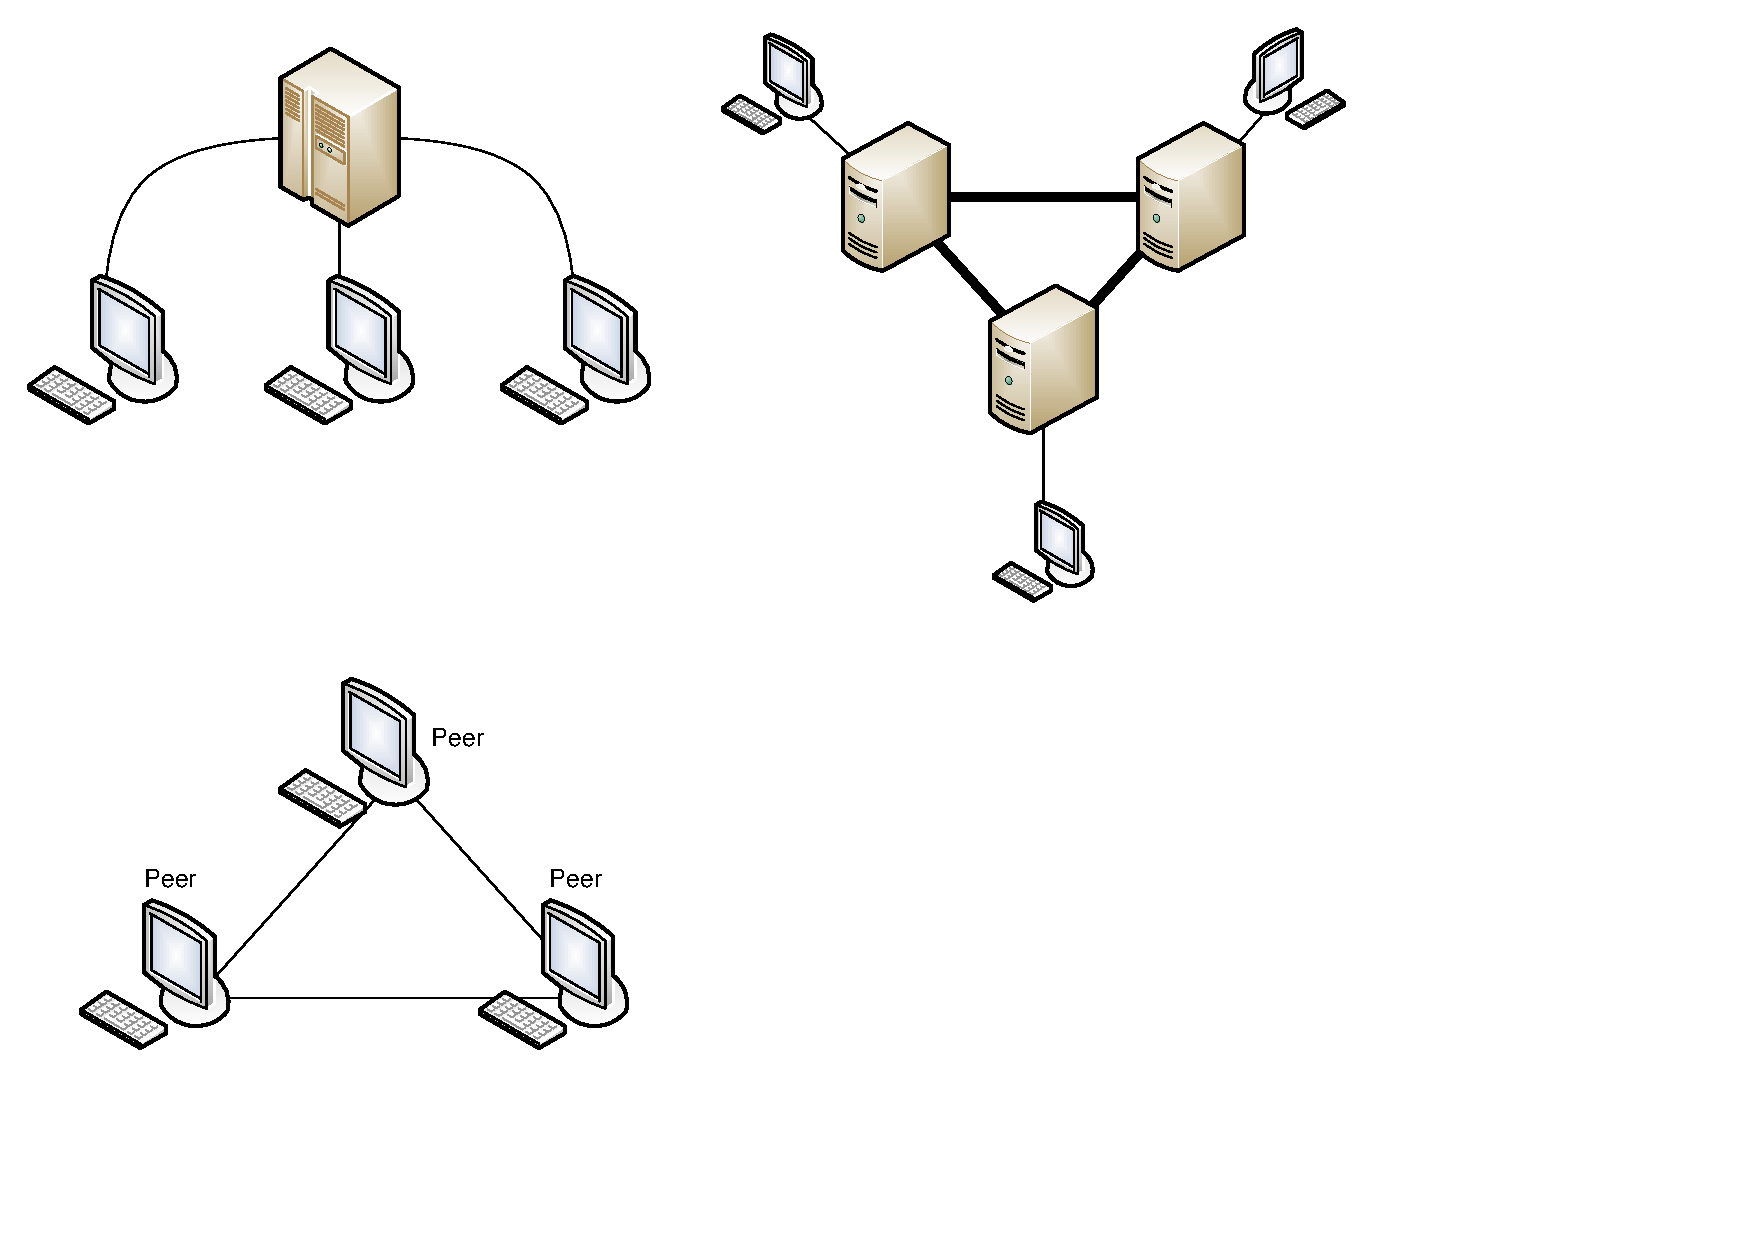
\includegraphics[clip=true, viewport= 1cm 3cm 12cm 10cm, width=0.5\columnwidth]{network_archs}
 \caption{Peer-to-Peer architecture}
 \label{fig_p2p_arch}
\end{figure}
%
Figure \ref{fig_p2p_arch} shows a peer-to-peer network architecture

\section{Conclusion}
The conclusion goes here.

\bibliographystyle{IEEEtran}
\bibliography{P2P_MMOG}

% that's all folks
\end{document}


